% !TEX root = ../SCXMLREF.tex


\subsection{Intrusion Detection System}
\label{sec:secbot}


The simple intrusion detection system is designed using an Application-Specific Integrated Circuit (ASIC) which connects to a buzzer and a sensor over a Serial Peripheral Interface (SPI) bus. The system is controlled via the ASIC on the SPI bus. At power-up, the ASIC sends commands over the SPI bus to initialize the sensor and the buzzer. After waiting for 50 milliseconds the ASIC enters its main routine, which makes the buzzer respond to the sensor. In the early design phase the statechart model of this system may be limited to the ASIC that captures the initialization of the peripherals and the 50 ms wait. In the interest of simplicity we elide all details of the main routine.

A statechart model of this system is shown in figure~\ref{fig:ASIC}. The ASIC starts by initializing the buzzer, this involves sending a message over the SPI bus. These messages constitute an implementation detail that we elide at this abstraction level. Once the message is sent (which will be indicated by some event saying that the SPI system is done), the ASIC moves on to initialize the sensor. After the ASIC moves into a waiting state for 50 ms, and finally moves into the state which represents normal operation. At this abstraction the \textbf{spi\_done} triggered, which signals completion by the SPI system, is an internal trigger that can be fired at any time.

\begin{figure*}[t!]
    % \begin{centering}
	    \begin{subfigure}[t]{0.5\textwidth}
	        \begin{centering}
	        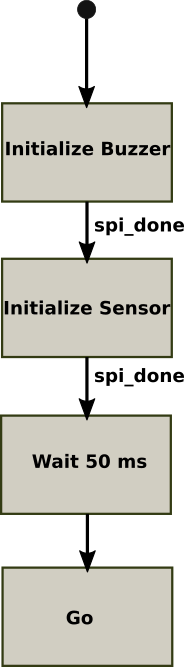
\includegraphics[height=3in]{figures/ASIC}
	        \caption{ASIC component high level abstraction}
	        \label{fig:ASIC}
	        \end{centering}
	    \end{subfigure}
\qquad
	    \begin{subfigure}[t]{0.5\textwidth}
	        % \begin{centering}
	        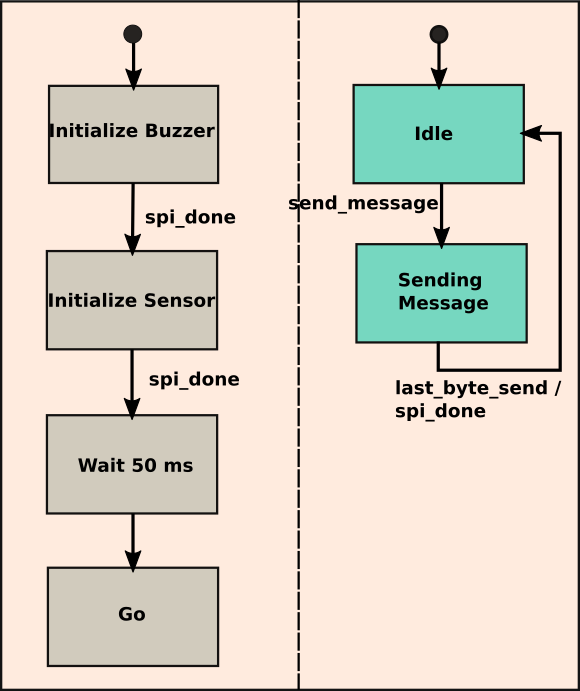
\includegraphics[height=3in]{figures/ASIC&SPI_1}
	        \caption{First refinement introducing the abstract model of the SPI subsystem.}
	        \label{fig:ASIC_SPI_1}
	        % \end{centering}
	    \end{subfigure}
	    \caption{Statechart diagram for Intrusion Detection System (SecBot) including the abstract representation of the ASIC and SPI components.}
    % \end{centering}
\end{figure*}

In a subsequent level of refinement, shown in figure~\ref{fig:ASIC_SPI_1}, the designer adds a parallel state representing the SPI subsystem. The SPI subsystem is usually on an \textbf{Idle} state until the \textbf{send\_message} trigger is raised, at which point the SPI subsystem enters a state \textbf{Sending Message}, which represents sending the message, byte by byte. When the last byte of the message is sent, it raises the \textbf{spi\_done} trigger, allowing the other parallel state to continue, while SPI subsystem returns to idle. In the current refined model the we have incorporated the implementation details for raising \textbf{spi\_done} and introduced a new internal trigger 
\textbf{send\_message}, which is nondeterministic at this point.

The model can be farther refined by incorporating more details on how the initialization states, the wait state, and the SPI subsystem operate, including how they interact with each other. The statechert diagram for this refinement level is in figure~\ref{fig:ASIC_SPI_2}. The \textbf{Initialize Buzzer} state constructs the SPI message to send, then raises the \textbf{send\_message} trigger, and then waits.
After \textbf{send\_message} is raised, the SPI subsystem reacts. It spins for a while in the \textbf{Send Byte} state, looping as many times as it takes to get to the last byte in the message. When the last byte in the message is sent, it goes back to \textbf{Idle} and raises an event which allows the state machine on the left to proceed. The sensor is then initialized in a very similar manner to the buzzer. After both peripherals are initialized, the state machine goes into the \textbf{Wait 50 ms} state, where it increments a counter until it reaches some maximum, then exits.

\begin{figure}[]
  \begin{centering}
  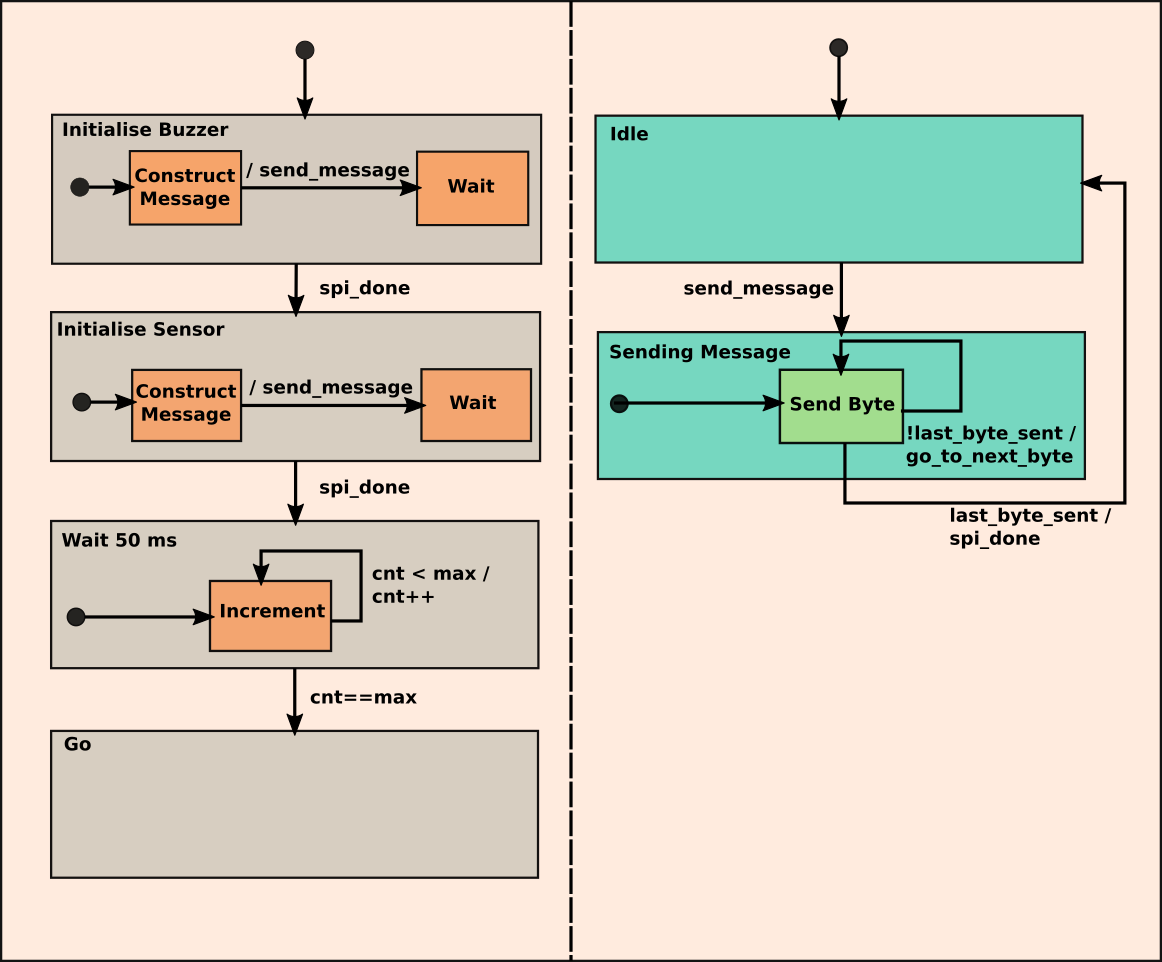
\includegraphics[width=0.8\textwidth]{figures/ASIC&SPI_2}
  \caption{Statechart diagram for Intrusion Detection System (SecBot) including implementation details for the messages send between the systems components.}
  \label{fig:ASIC_SPI_2}
  \end{centering}
\end{figure} 

The system described must send messages to complete the initialization of the buzzer and sensor, but once the main routine is reached (\textbf{Go} state) no more messages should be sent through the SPI bus. As a result, when the ASIC is in the \textbf{Go} state the SPI subsystem must be in the \textbf{Idle} state. This system property must be satisfied by the system model first refinement and any subsequent refinement representations of the system.

% \begin{lstlisting}[caption=Snippet for SCXML representation of SecBot model,label={lst:secBot}, language=xml]
% ...
% <state id="SecBot" iumlb:refinement="0">
%     <parallel id="SecBot_parallel">

%      	<!-- For ASIC component -->
%     	<state id="ASIC" iumlb:refinement="0">
%         	<initial iumlb:refinement="0">
%           		<transition target="InitialiseBuzzer"/>
%         	</initial>
%         	<state id="InitialiseBuzzer" iumlb:refinement="2">
%         		<initial iumlb:refinement="2">
% 	            	<transition target="IBConstructMessage"/>
% 	          	</initial>
%           		<transition cond="" event="spi_done" target="InitialiseSensor"/>
%           		<state id="IBConstructMessage" iumlb:refinement="2">
% 	            	<transition target="IBWait">
% 	              		<raise event="send_message"/>
% 	            	</transition>
%           		</state>
%           		<state id="IBWait" iumlb:refinement="2"/>
%         	</state>
%        		<state id="InitialiseSensor" iumlb:refinement="2">
%         		...
%         	</state>
%         	<state id="Wait50ms" iumlb:refinement="2">
%           		...
%         	</state>
%         	<state id="Go">
%           		<iumlb:invariant name="spi_idle_in_Go" iumlb:predicate="Idle = TRUE" iumlb:refinement="1"/>
%         	</state>
%       	</state>

%       	<!-- For SPI subsystem -->
%       	<state id="SPI" iumlb:refinement="1">
% 	        <initial>
% 	        	<transition target="Idle"/>
% 	        </initial>
% 	        <state id="Idle">
% 				<transition event="send_message" target="SendingMessage">
% 					<iumlb:guard name="dontRaiseSpiDone" iumlb:predicate="spi_done ∉ SCXML_raisedTriggers" iumlb:refinement="1"/>
% 				</transition>
%         	</state>
% 			<state id="SendingMessage">
% 				<transition cond="" event="last_byte_sent" target="Idle">
% 					<raise event="spi_done"/>
% 					<iumlb:guard name="dontRaiseSendMessage" iumlb:predicate="send_message ∉ SCXML_raisedTriggers" iumlb:refinement="1"/>
% 				</transition>
% 			</state>
% 		</state>
% 	</parallel>
% </state>
% ...
% \end{lstlisting}






